\documentclass[aspectratio=169]{beamer}

% =================================================================
%  Automation in Marine Industry
%  A beginner-friendly Beamer deck (fully self-contained: all
%  figures / flowcharts / plots drawn with TikZ, so it compiles anywhere).
% =================================================================

% -------------------------------------------------
% Theme and packages
% -------------------------------------------------
\usetheme{Madrid}
\usecolortheme{default}

\usepackage{amsmath}
\usepackage{amssymb}
\usepackage{bm}
\usepackage{listings}
\usepackage{tikz}
\usepackage{array}
\usepackage{booktabs}
\usepackage{tabularx}
\usepackage{ragged2e}
\usepackage{xcolor}

\usetikzlibrary{shapes.geometric, arrows.meta, positioning, calc, fit, backgrounds, patterns}

% -------------------------------------------------
% Colour palette
% -------------------------------------------------
\definecolor{cAccent}{RGB}{0,102,153}     % teal-blue accent
\definecolor{cBox}{RGB}{28,31,42}          % dark box
\definecolor{cGreen}{RGB}{34,139,34}
\definecolor{cRed}{RGB}{178,34,34}
\definecolor{cOrange}{RGB}{204,102,0}
\definecolor{cPurple}{RGB}{102,45,145}
\definecolor{cGrayBg}{RGB}{245,246,248}
\definecolor{codebg}{RGB}{248,248,244}
\definecolor{codekw}{RGB}{0,0,180}
\definecolor{codecomment}{RGB}{0,130,0}
\definecolor{codestr}{RGB}{170,55,20}

% Beamer colour tweaks (match a Madrid-style accent)
\setbeamercolor{structure}{fg=cAccent}
\setbeamertemplate{frametitle continuation}{%
	\ifnum\insertcontinuationcount>1\space(cont...)\fi
}
\setbeamertemplate{navigation symbols}{}
\setbeamertemplate{caption}[numbered]

% -------------------------------------------------
% Listings style for C code
% -------------------------------------------------
\lstdefinestyle{cstyle}{
	language=C,
	backgroundcolor=\color{codebg},
	basicstyle=\ttfamily\footnotesize,
	keywordstyle=\color{codekw}\bfseries,
	commentstyle=\color{codecomment}\itshape,
	stringstyle=\color{codestr},
	numbers=none,
	numberstyle=\tiny\color{gray},
	numbersep=8pt,
	showstringspaces=false,
	breaklines=true,
	frame=single,
	rulecolor=\color{gray!50},
	tabsize=2,
	columns=fullflexible,
	keepspaces=true,
	literate={~}{{$\sim$}}1
}
\lstset{style=cstyle}

% Handy TikZ flowchart node styles
\tikzset{
	startstop/.style={rectangle, rounded corners=10pt, minimum width=2.4cm, minimum height=0.8cm, text centered, align=center, draw=black, fill=cAccent!25},
	process/.style  ={rectangle, minimum width=2.6cm, minimum height=0.8cm, text centered, align=center, text width=2.8cm, draw=black, fill=blue!8},
	io/.style       ={trapezium, trapezium left angle=70, trapezium right angle=110, minimum width=2.2cm, minimum height=0.8cm, text centered, align=center, draw=black, fill=cOrange!20},
	decision/.style ={diamond, aspect=2, minimum width=2.4cm, minimum height=0.9cm, text centered, text width=2.2cm, draw=black, fill=cGreen!18, inner sep=1pt},
	flowarrow/.style={-{Stealth[length=2.5mm]}, thick},
	% block diagram styles
	blk/.style      ={rectangle, draw=black, thick, minimum width=1.9cm, minimum height=0.9cm, align=center, fill=blue!8},
	sig/.style      ={-{Stealth[length=2.2mm]}, thick},
	% robot drawing styles
	link/.style     ={line width=4pt, cOrange, line cap=round},
	joint/.style    ={circle, draw=black, thick, fill=white, minimum size=0.28cm, inner sep=0pt},
}

\setbeamertemplate{footnote}{%
	\parindent 0em
	\noindent
	\raggedright
	\insertfootnotemark\insertfootnotetext\par
}

% -------------------------------------------------
% Title information
% -------------------------------------------------
\title[Automation in Marine Industry]{Automation in Marine Industry}
\subtitle{Manufacturing Concepts, Shipbuilding Automation, Digital Shipyards \& Robotics}
\author[Amit Kumar Singh]{}
\institute[]{
	Amit Kumar Singh \\
	\vspace{0.1cm}
	Assistant Professor (ECE) \\
	\vspace{0.05cm}
	School of Naval Architecture and Ocean Engineering\\
	\vspace{0.05cm}
	Indian Maritime University Visakhapatnam Campus, Sabbavaram Mandal\\
	\vspace{0.05cm}
	Visakhapatnam, Andhra Pradesh -- 531~035\\
	\vspace{0.25cm}
	amitkumarsingh@imu.ac.in
}
\date[AI \& Automation]{\today}

\begin{document}

	%------------------------------------------------
	\begin{frame}
		\titlepage
	\end{frame}

	%------------------------------------------------
	\begin{frame}{Outline}
		\small
		\begin{columns}[T,onlytextwidth]
			\hspace{0.8cm}% shift the first column to the right
			\begin{column}{0.49\textwidth}
				\tableofcontents[hideallsubsections, sections={1-6}]
			\end{column}
			\hspace{0.8cm}% wider gap between the two columns
			\begin{column}{0.40\textwidth}
				\tableofcontents[hideallsubsections, sections={7-11}]
			\end{column}
		\end{columns}
	\end{frame}

	% =================================================================
	\section{Concepts in Manufacturing and Automation}
	% =================================================================
	\begin{frame}{What is Manufacturing?}
		\begin{block}{Two views of manufacturing}
			\textbf{Technological:} applying physical and chemical processes to change the geometry, properties or appearance of a material to make parts or products.\\[3pt]
			\textbf{Economic:} transforming materials into items of \textbf{greater value} by processing and assembly --- \emph{value is added}.
		\end{block}
		\begin{columns}
			\begin{column}{0.58\textwidth}
				\begin{itemize}\small
					\item Four basic \textbf{manufacturing operations}:
					\begin{enumerate}\footnotesize
						\item \textbf{Processing} --- cutting, bending, welding, painting.
						\item \textbf{Assembly} --- joining parts into blocks, blocks into a hull.
						\item \textbf{Material handling} --- cranes, transporters, conveyors.
						\item \textbf{Inspection \& test} --- NDT, dimensional checks, sea trials.
					\end{enumerate}
				\end{itemize}
			\end{column}
			\begin{column}{0.42\textwidth}
				\centering
				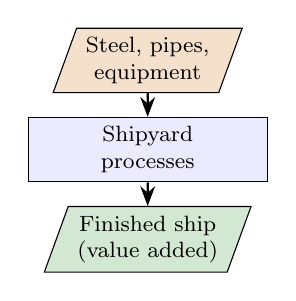
\begin{tikzpicture}[node distance=0.3cm, every node/.style={font=\footnotesize}]
					\node[io, fill=cOrange!20] (in) {Steel, pipes,\\ equipment};
					\node[process, below=of in] (proc) {Shipyard\\ processes};
					\node[io, below=of proc, fill=cGreen!20] (out) {Finished ship\\ (value added)};
					\draw[flowarrow] (in) -- (proc);
					\draw[flowarrow] (proc) -- (out);
				\end{tikzpicture}
			\end{column}
		\end{columns}
	\end{frame}

	\begin{frame}{The Production System}
		\centering
		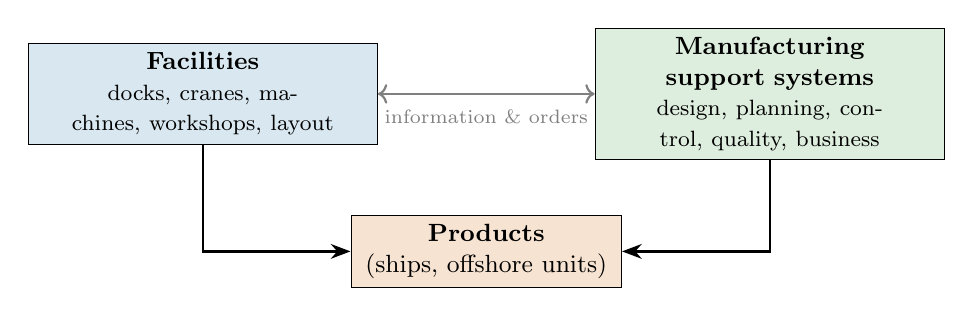
\begin{tikzpicture}[font=\small]
			\node[process, fill=cAccent!15, text width=4.2cm, minimum height=1.2cm] (fac) at (-3.6,0) {\textbf{Facilities}\\ \footnotesize docks, cranes, machines, workshops, layout};
			\node[process, fill=cGreen!15, text width=4.2cm, minimum height=1.2cm] (sup) at (3.6,0) {\textbf{Manufacturing support systems}\\ \footnotesize design, planning, control, quality, business};
			\node[process, fill=cOrange!18, text width=3.2cm] (pr) at (0,-2.0) {\textbf{Products}\\ (ships, offshore units)};
			\draw[flowarrow] (fac) |- (pr);
			\draw[flowarrow] (sup) |- (pr);
			\draw[<->, thick, gray] (fac) -- node[below=2pt, font=\scriptsize, text=gray] {information \& orders} (sup);
		\end{tikzpicture}
		\vspace{0.3cm}
		\begin{columns}[T]
			\begin{column}{0.5\textwidth}
				\begin{block}{Automation of facilities}
					\small CNC cutting, welding robots, automatic panel lines, crane control --- \textbf{automated manufacturing systems}.
				\end{block}
			\end{column}
			\begin{column}{0.5\textwidth}
				\begin{block}{Computerised support systems}
					\small CAD/CAM, production planning, ERP, MES --- \textbf{computer-integrated manufacturing (CIM)}.
				\end{block}
			\end{column}
		\end{columns}
	\end{frame}

	\begin{frame}{Production Metrics: Worked Examples}
		\begin{columns}[T]
			\begin{column}{0.5\textwidth}
				\begin{block}{Key definitions}
					\small
					\textbf{Cycle time} $T_c$ --- time per part at a station.\\
					\textbf{Production rate} $R_p = 60/T_c$ (parts/h).\\
					\textbf{Availability} $A = \dfrac{\text{MTBF} - \text{MTTR}}{\text{MTBF}}$\\[3pt]
					\textbf{Manufacturing lead time}\\
					$\text{MLT} = n_o\left(\dfrac{T_{su}}{Q} + T_c + T_{no}\right)$
				\end{block}
				\footnotesize $n_o$ = operations, $T_{su}$ = set-up time, $Q$ = batch size, $T_{no}$ = non-operation (waiting, moving) time.
			\end{column}
			\begin{column}{0.5\textwidth}
				\small
				\textbf{1.} A stiffener-cutting station has $T_c = 6$ min:\\
				$R_p = 60/6 = \boxed{10\ \text{parts/h}}$
				\vspace{0.15cm}

				\textbf{2.} A plasma cutter: MTBF $= 50$ h, MTTR $= 5$ h:\\
				$A = (50 - 5)/50 = \boxed{0.90}$
				\vspace{0.15cm}

				\textbf{3.} A batch of $Q = 20$ panels passes $n_o = 4$ operations, each with $T_{su} = 3$ h, $T_c = 0.5$ h, $T_{no} = 6$ h:\\
				$\text{MLT} = 4\,(0.15 + 0.5 + 6) = \boxed{26.6\ \text{h}}$
				\vspace{0.1cm}

				\footnotesize Waiting time dominates --- automation of \emph{handling} and \emph{planning} often saves more than faster machines.
			\end{column}
		\end{columns}
	\end{frame}

	\begin{frame}{What is Automation?}
		\begin{block}{Automation}
			Technology by which a process or procedure is performed with \textbf{minimum human assistance}, using \textbf{power}, a \textbf{program of instructions} and a \textbf{control system}.
		\end{block}
		\vspace{0.1cm}
		\begin{columns}[T]
			\begin{column}{0.55\textwidth}
				\begin{itemize}\small
					\item \textbf{Mechanisation} --- machines replace human \emph{muscle} (a powered welding carriage).
					\item \textbf{Automation} --- machines also replace human \emph{control and decisions} (a robot that finds and welds the seam itself).
					\item \textbf{Computerisation} --- information flow is automated (CAD model $\rightarrow$ robot program).
				\end{itemize}
			\end{column}
			\begin{column}{0.45\textwidth}
				\centering
				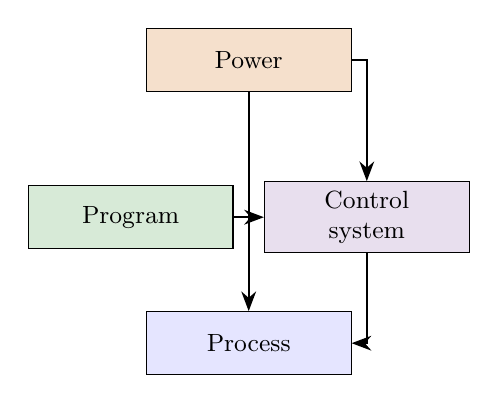
\begin{tikzpicture}[font=\small]
					\node[process, fill=cOrange!20, text width=2.0cm] (pw) at (0,2.0) {Power};
					\node[process, fill=cGreen!18, text width=2.0cm] (pg) at (-1.5,0) {Program};
					\node[process, fill=cPurple!15, text width=2.0cm] (cs) at (1.5,0) {Control\\ system};
					\node[process, fill=blue!10, text width=2.0cm] (pr) at (0,-1.6) {Process};
					\draw[flowarrow] (pw) -- (pr);
					\draw[flowarrow] (pg) -- (cs);
					\draw[flowarrow] (cs) |- (pr);
					\draw[flowarrow] (pw) -| (cs);
				\end{tikzpicture}
			\end{column}
		\end{columns}
	\end{frame}

	% =================================================================
	\section{Reasons for Automating}
	% =================================================================
	\begin{frame}{Reasons for Automating}
		\begin{columns}[T]
			\begin{column}{0.5\textwidth}
				\begin{block}{General reasons}
					\begin{itemize}\small
						\item Increase labour \textbf{productivity}.
						\item Reduce labour cost; overcome labour \textbf{shortages}.
						\item Reduce or remove routine manual tasks.
						\item Improve worker \textbf{safety}.
						\item Improve product \textbf{quality}.
						\item Reduce manufacturing \textbf{lead time}.
						\item Do what cannot be done manually.
						\item Avoid the high cost of \emph{not} automating.
					\end{itemize}
				\end{block}
			\end{column}
			\begin{column}{0.5\textwidth}
				\begin{block}{Especially in shipbuilding}
					\begin{itemize}\small
						\item Shortage of \textbf{skilled welders} and fitters.
						\item Welding in \textbf{confined} double-bottom cells and tanks --- heat, fumes.
						\item Blasting \& painting --- dust, solvents, health hazards.
						\item Tight delivery schedules and global price competition.
						\item Class \& coating rules demand documented, consistent quality.
					\end{itemize}
				\end{block}
			\end{column}
		\end{columns}
	\end{frame}

	\begin{frame}{The Case For and Against Automation}
		\renewcommand{\arraystretch}{1.3}
		\centering
		\small
		\begin{tabular}{@{}>{\raggedright}p{6.0cm}>{\raggedright\arraybackslash}p{6.6cm}@{}}
			\toprule
			\textbf{For} & \textbf{Against / cautions} \\
			\midrule
			Higher output per worker and per shift     & High capital cost; long payback for low volumes \\
			Consistent weld and paint quality          & Every ship is different --- programming effort \\
			Safer, healthier working conditions        & Large, heavy, curved parts are hard to fixture \\
			Better data for planning and costing       & Needs skilled technicians \& maintenance \\
			Competitiveness against low-wage yards     & Workforce concerns --- retraining required \\
			\bottomrule
		\end{tabular}
		\vspace{0.3cm}
		\begin{block}{The USA principle}
			\small \textbf{U}nderstand the existing process $\rightarrow$ \textbf{S}implify it $\rightarrow$ \textbf{A}utomate it. In shipbuilding, simplification (standard details, straight panels, fewer part types) is often the biggest step.
		\end{block}
	\end{frame}

	% =================================================================
	\section{Types of Production}
	% =================================================================
	\begin{frame}{Types of Production}
		\begin{columns}[T]
			\begin{column}{0.32\textwidth}
				\begin{block}{Low quantity (job shop)}
					\centering
					\textbf{1--100 units / year}

					\vspace{0.2cm}

					\begin{itemize}\small
						\item Special, customised products.
						\item General-purpose equipment.
						\item \textbf{Ships}, offshore units.
					\end{itemize}
				\end{block}
			\end{column}
			\begin{column}{0.32\textwidth}
				\begin{block}{Medium quantity (batch)}
					\centering
					\textbf{100--10\,000 / year}

					\vspace{0.2cm}

					\begin{itemize}\small
						\item Batches, then change-over.
						\item Cells for part families.
						\item Engines, pumps, boats.
					\end{itemize}
				\end{block}
			\end{column}
			\begin{column}{0.32\textwidth}
				\begin{block}{High quantity (mass)}
					\centering
					\textbf{$>$ 10\,000 / year}

					\vspace{0.2cm}

					\begin{itemize}\small
						\item Flow-line production.
						\item Special-purpose equipment.
						\item Fasteners, cars.
					\end{itemize}
				\end{block}
			\end{column}
		\end{columns}
		\vspace{0.05cm}
		\centering
		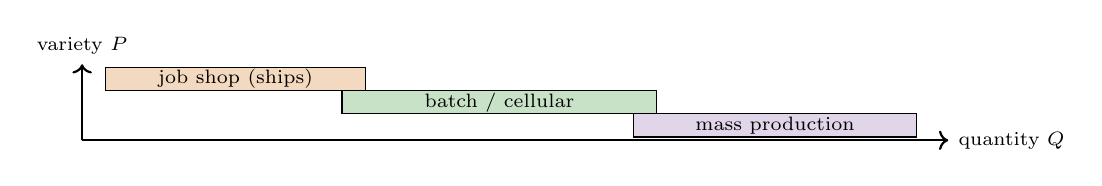
\begin{tikzpicture}[font=\scriptsize, x=1.0cm, y=0.42cm]
			\draw[->, thick] (0,0) -- (11,0) node[right] {quantity $Q$};
			\draw[->, thick] (0,0) -- (0,2.3) node[above] {variety $P$};
			\filldraw[fill=cOrange!25, draw=black] (0.3,1.5) rectangle (3.6,2.2);
			\node at (1.95,1.85) {job shop (ships)};
			\filldraw[fill=cGreen!25, draw=black] (3.3,0.8) rectangle (7.3,1.5);
			\node at (5.3,1.15) {batch / cellular};
			\filldraw[fill=cPurple!20, draw=black] (7.0,0.1) rectangle (10.6,0.8);
			\node at (8.8,0.45) {mass production};
		\end{tikzpicture}
	\end{frame}

	\begin{frame}{Where Does Shipbuilding Fit?}
		\begin{columns}[T]
			\begin{column}{0.55\textwidth}
				\begin{block}{A paradox}
					\small The \textbf{ship} is a one-off (job-shop) product, but it is made from \textbf{thousands of similar parts}: plates, stiffeners, brackets, pipe spools, panels.
				\end{block}
				\begin{itemize}\small
					\item \textbf{Group technology}: group similar interim products into families (flat panels, curved blocks, pipe spools).
					\item Each family is built on a dedicated \textbf{work station or line} --- batch-like and automatable.
					\item Result: a \emph{job-shop product} built with \emph{flow-line methods}.
				\end{itemize}
			\end{column}
			\begin{column}{0.45\textwidth}
				\renewcommand{\arraystretch}{1.25}
				\centering
				\small
				\begin{tabular}{@{}lr@{}}
					\toprule
					\textbf{Item in one ship} & \textbf{Approx.\ count} \\
					\midrule
					Steel parts        & 20\,000--50\,000 \\
					Flat panels        & 100--300 \\
					Hull blocks        & 50--200 \\
					Pipe spools        & 5\,000--15\,000 \\
					Weld length        & 100s of km \\
					\bottomrule
				\end{tabular}
				\vspace{0.1cm}

				\footnotesize Indicative figures for a large merchant ship.
			\end{column}
		\end{columns}
	\end{frame}

	\begin{frame}{Plant Layouts in a Shipyard}
		\renewcommand{\arraystretch}{1.3}
		\centering
		\small
		\begin{tabular}{@{}>{\raggedright}p{2.8cm}>{\raggedright}p{4.6cm}>{\raggedright\arraybackslash}p{5.2cm}@{}}
			\toprule
			\textbf{Layout} & \textbf{Idea} & \textbf{Shipyard example} \\
			\midrule
			Fixed-position   & product stays; workers \& equipment come to it & hull erection in the building dock \\
			Process          & machines grouped by process type & plate shop, pipe shop, paint shop \\
			Cellular         & cells dedicated to part families & sub-assembly cells, pipe-spool cells \\
			Product (flow line) & stations in sequence; work flows through & \textbf{automatic panel line} \\
			\bottomrule
		\end{tabular}
		\vspace{0.3cm}
		\begin{block}{Key idea}
			\small Modern yards move as much work as possible \textbf{upstream} --- from the dock (fixed-position, hard to automate) into workshops with cellular and flow-line layouts (easy to automate).
		\end{block}
	\end{frame}

	% =================================================================
	\section{Types of Automation}
	% =================================================================
	\begin{frame}{Types of Automation}
		\begin{columns}[T]
			\begin{column}{0.32\textwidth}
				\begin{block}{Fixed}
					\centering
					\textbf{Hard automation}

					\vspace{0.2cm}

					\begin{itemize}\small
						\item Sequence fixed by equipment design.
						\item High volume, one product.
						\item \textbf{Yard}: shot-blasting \& priming line for plates, profile cutting line.
					\end{itemize}
				\end{block}
			\end{column}
			\begin{column}{0.32\textwidth}
				\begin{block}{Programmable}
					\centering
					\textbf{Change the program}

					\vspace{0.2cm}

					\begin{itemize}\small
						\item New part = new program.
						\item Batch production.
						\item \textbf{Yard}: CNC plasma cutting, robot welding of sub-assemblies.
					\end{itemize}
				\end{block}
			\end{column}
			\begin{column}{0.32\textwidth}
				\begin{block}{Flexible}
					\centering
					\textbf{No change-over loss}

					\vspace{0.2cm}

					\begin{itemize}\small
						\item Mix of different parts.
						\item Programs made off-line.
						\item \textbf{Yard}: panel line with robots programmed automatically from CAD.
					\end{itemize}
				\end{block}
			\end{column}
		\end{columns}
		\vspace{0.3cm}
		\begin{block}{Which fits shipbuilding?}
			\small Because every ship is different, shipyards rely mainly on \textbf{programmable and flexible} automation --- and on getting the robot programs \textbf{directly from the 3-D product model}.
		\end{block}
	\end{frame}

	% =================================================================
	\section{Automation Strategies}
	% =================================================================
	\begin{frame}{Ten Strategies for Automation and Process Improvement}
		\renewcommand{\arraystretch}{1.12}
		\centering
		\footnotesize
		\begin{tabular}{@{}rp{5.0cm}p{7.4cm}@{}}
			\toprule
			\textbf{\#} & \textbf{Strategy} & \textbf{Shipyard example} \\
			\midrule
			1  & Specialisation of operations    & dedicated stiffener-welding gantry \\
			2  & Combined operations              & cut, mark and bevel a plate in one CNC set-up \\
			3  & Simultaneous operations          & several welding heads on one panel at once \\
			4  & Integration of operations        & plate line: blasting $\to$ priming $\to$ cutting linked by conveyors \\
			5  & Increased flexibility            & robots programmed per panel from CAD \\
			6  & Improved material handling       & block transporters, automated plate stock-yard \\
			7  & On-line inspection               & laser scanning of block dimensions (accuracy control) \\
			8  & Process control \& optimisation  & adaptive welding with seam tracking \\
			9  & Plant operations control         & MES tracking every block and pipe spool \\
			10 & Computer-integrated manufacturing & one product model from design to delivery (\emph{digital shipyard}) \\
			\bottomrule
		\end{tabular}
	\end{frame}

	\begin{frame}{Automation Migration Strategy}
		\begin{block}{Step-by-step path}
			New products or processes are rarely automated in one step. The \textbf{migration strategy} moves from manual to fully integrated production as demand and experience grow.
		\end{block}
		\centering
		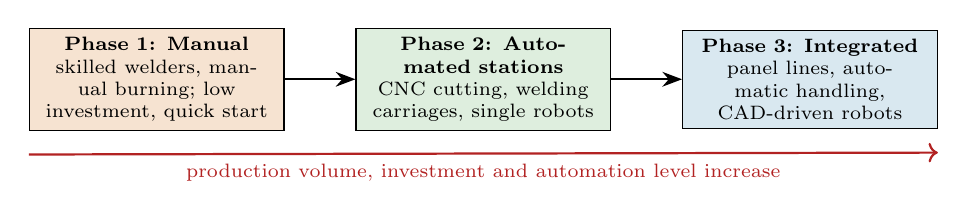
\begin{tikzpicture}[every node/.style={font=\scriptsize}, node distance=0.9cm]
			\node[process, fill=cOrange!18, text width=3.0cm] (p1) {\textbf{Phase 1: Manual}\\ skilled welders, manual burning; low investment, quick start};
			\node[process, right=of p1, fill=cGreen!15, text width=3.0cm] (p2) {\textbf{Phase 2: Automated stations}\\ CNC cutting, welding carriages, single robots};
			\node[process, right=of p2, fill=cAccent!15, text width=3.0cm] (p3) {\textbf{Phase 3: Integrated}\\ panel lines, automatic handling, CAD-driven robots};
			\draw[flowarrow] (p1) -- (p2);
			\draw[flowarrow] (p2) -- (p3);
			\draw[->, thick, cRed] ($(p1.south west)+(0,-0.3)$) -- ($(p3.south east)+(0,-0.3)$) node[midway, below] {production volume, investment and automation level increase};
		\end{tikzpicture}
		\vspace{0.3cm}
		\begin{itemize}\small
			\item Reduces risk --- each step is proven before the next investment.
			\item Uses the same product model data at every phase so programs and experience carry forward.
		\end{itemize}
	\end{frame}

	% =================================================================
	\section{Levels of Automation in Shipbuilding}
	% =================================================================
	\begin{frame}{The Shipbuilding Production Process}
		\centering
		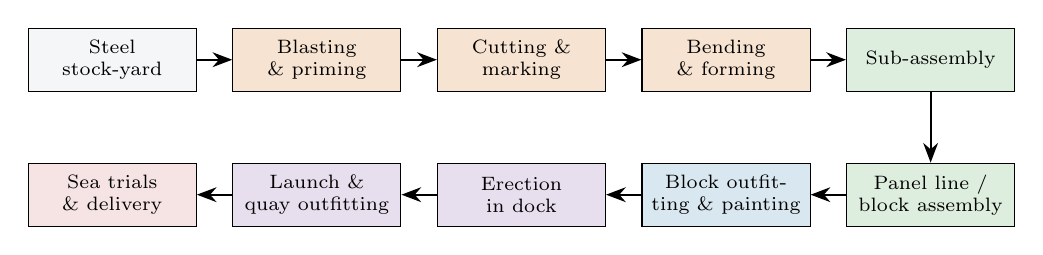
\begin{tikzpicture}[every node/.style={font=\scriptsize}, node distance=0.45cm,
			st/.style={process, minimum width=1.9cm, text width=1.9cm, minimum height=0.8cm}]
			\node[st, fill=cGrayBg] (s1) {Steel stock-yard};
			\node[st, right=of s1, fill=cOrange!18] (s2) {Blasting \& priming};
			\node[st, right=of s2, fill=cOrange!18] (s3) {Cutting \& marking};
			\node[st, right=of s3, fill=cOrange!18] (s4) {Bending \& forming};
			\node[st, right=of s4, fill=cGreen!15] (s5) {Sub-assembly};
			\node[st, below=0.9cm of s5, fill=cGreen!15] (s6) {Panel line / block assembly};
			\node[st, left=of s6, fill=cAccent!15] (s7) {Block outfitting \& painting};
			\node[st, left=of s7, fill=cPurple!15] (s8) {Erection in dock};
			\node[st, left=of s8, fill=cPurple!15] (s9) {Launch \& quay outfitting};
			\node[st, left=of s9, fill=cRed!12] (s10) {Sea trials \& delivery};
			\draw[flowarrow] (s1) -- (s2); \draw[flowarrow] (s2) -- (s3); \draw[flowarrow] (s3) -- (s4); \draw[flowarrow] (s4) -- (s5);
			\draw[flowarrow] (s5) -- (s6); \draw[flowarrow] (s6) -- (s7); \draw[flowarrow] (s7) -- (s8); \draw[flowarrow] (s8) -- (s9); \draw[flowarrow] (s9) -- (s10);
		\end{tikzpicture}
		\vspace{0.3cm}
		\begin{columns}[T]
			\begin{column}{0.5\textwidth}
				\begin{block}{Hull block construction (HBCM)}
					\small The hull is divided into \textbf{blocks} (50--900 t) built in parallel in workshops, then \textbf{erected} in the dock.
				\end{block}
			\end{column}
			\begin{column}{0.5\textwidth}
				\begin{block}{Zone outfitting \& painting}
					\small Pipes, cables and equipment are fitted and blocks are painted \textbf{before} erection --- easier access, less work in the dock.
				\end{block}
			\end{column}
		\end{columns}
	\end{frame}

	\begin{frame}{Levels of Automation (Degree of Automation)}
		\centering
		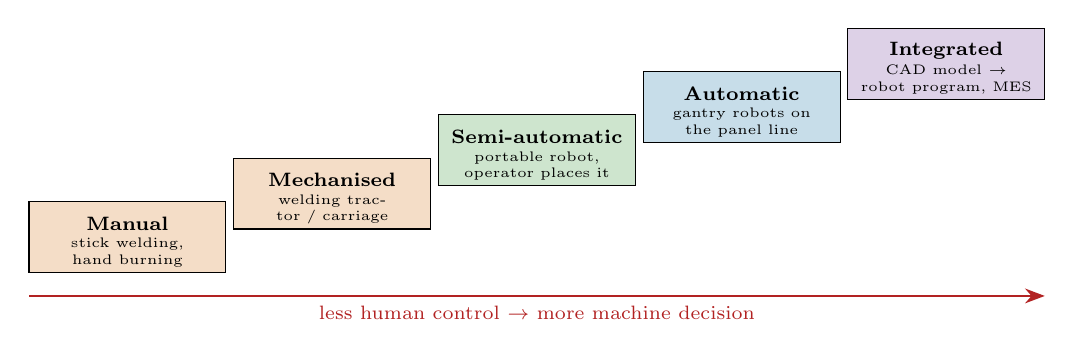
\begin{tikzpicture}[font=\scriptsize]
			\foreach \i/\t/\d/\c in {
				0/{Manual}/{stick welding, hand burning}/cOrange,
				1/{Mechanised}/{welding tractor / carriage}/cOrange,
				2/{Semi-automatic}/{portable robot, operator places it}/cGreen,
				3/{Automatic}/{gantry robots on the panel line}/cAccent,
				4/{Integrated}/{CAD model $\to$ robot program, MES}/cPurple} {
				\filldraw[fill=\c!22, draw=black] ({\i*2.6},{\i*0.55}) rectangle ({\i*2.6+2.5},{\i*0.55+0.9});
				\node[font=\scriptsize\bfseries] at ({\i*2.6+1.25},{\i*0.55+0.62}) {\t};
				\node[text width=2.3cm, align=center, font=\tiny] at ({\i*2.6+1.25},{\i*0.55+0.25}) {\d};
			}
			\draw[flowarrow, cRed] (0,-0.3) -- (12.9,-0.3) node[midway, below] {less human control $\rightarrow$ more machine decision};
		\end{tikzpicture}
		\vspace{0.3cm}
		\begin{columns}[T]
			\begin{column}{0.5\textwidth}
				\begin{block}{Hierarchy levels}
					\small \textbf{Device} (sensor, motor) $\to$ \textbf{machine} (robot, CNC) $\to$ \textbf{cell / line} (panel line) $\to$ \textbf{plant} (yard MES) $\to$ \textbf{enterprise} (ERP, supply chain).
				\end{block}
			\end{column}
			\begin{column}{0.5\textwidth}
				\begin{block}{Rule of thumb}
					\small The more \textbf{repetitive} and \textbf{flat / straight} the work, the higher the level of automation that pays off.
				\end{block}
			\end{column}
		\end{columns}
	\end{frame}

	\begin{frame}{Level of Automation by Production Stage}
		\begin{columns}[T]
			\begin{column}{0.58\textwidth}
				\centering
				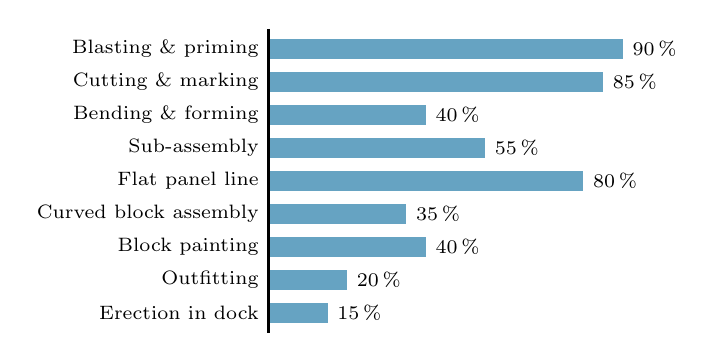
\begin{tikzpicture}[font=\scriptsize, x=0.05cm, y=0.42cm]
					\foreach \n/\v/\l in {
						0/90/{Blasting \& priming},
						1/85/{Cutting \& marking},
						2/40/{Bending \& forming},
						3/55/{Sub-assembly},
						4/80/{Flat panel line},
						5/35/{Curved block assembly},
						6/40/{Block painting},
						7/20/{Outfitting},
						8/15/{Erection in dock}} {
						\pgfmathsetmacro{\yy}{-\n}
						\node[left] at (0,\yy) {\l};
						\fill[cAccent!60] (0,\yy-0.3) rectangle (\v,\yy+0.3);
						\node[right] at (\v,\yy) {\v\,\%};
					}
					\draw[thick] (0,0.6) -- (0,-8.6);
				\end{tikzpicture}

				\footnotesize Indicative degree of automation in a modern yard.
			\end{column}
			\begin{column}{0.42\textwidth}
				\begin{itemize}\small
					\item \textbf{Highest} where parts are flat, straight and repeated: plate lines, cutting, flat panels.
					\item \textbf{Lowest} where work is 3-D, confined or unique: curved blocks, outfitting, erection.
					\item Research focus: mobile robots for \textbf{confined spaces} and \textbf{erection joints}.
				\end{itemize}
			\end{column}
		\end{columns}
	\end{frame}

	% =================================================================
	\section{Digital Shipyards}
	% =================================================================
	\begin{frame}{What is a Digital Shipyard?}
		\begin{block}{Digital shipyard (Shipyard 4.0)}
			A shipyard where design, planning, production and after-sales share \textbf{one digital product model} and \textbf{real-time data}, connected by networks, sensors and software --- Industry 4.0 applied to shipbuilding.
		\end{block}
		\begin{columns}[T]
			\begin{column}{0.5\textwidth}
				\begin{itemize}\small
					\item \textbf{3-D product model} --- single source for drawings, part lists, NC and robot programs.
					\item \textbf{Digital twin} --- virtual copy of the ship and of the yard, updated with real data.
					\item \textbf{IoT \& RFID} --- track plates, blocks, pipe spools, tools and people.
					\item \textbf{Simulation} --- test the production plan before cutting steel.
				\end{itemize}
			\end{column}
			\begin{column}{0.5\textwidth}
				\begin{itemize}\small
					\item \textbf{MES / ERP} --- plan and follow every work package.
					\item \textbf{AR / VR} --- workers see the model overlaid on the real block.
					\item \textbf{3-D laser scanning} --- compare built blocks with the model (accuracy control).
					\item \textbf{Data analytics \& AI} --- predict delays, optimise crane use.
				\end{itemize}
			\end{column}
		\end{columns}
	\end{frame}

	\begin{frame}{The Digital Thread in a Shipyard}
		\centering
		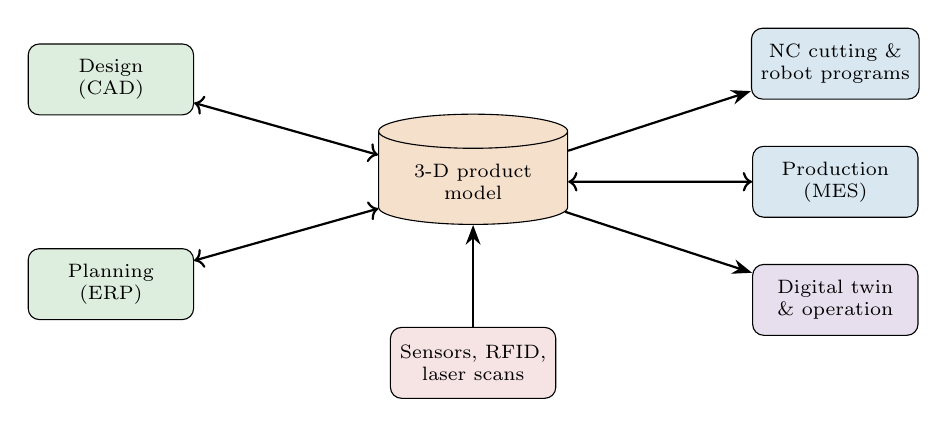
\begin{tikzpicture}[every node/.style={font=\scriptsize},
			tool/.style={rectangle, draw=black, rounded corners, minimum width=2.1cm, minimum height=0.9cm, align=center, fill=blue!10}]
			\node[cylinder, draw=black, shape border rotate=90, aspect=0.25, minimum width=2.4cm, minimum height=1.4cm, fill=cOrange!20, align=center] (pm) at (0,0) {3-D product\\ model};
			\node[tool, fill=cGreen!15] (des) at (-4.6,1.3) {Design\\ (CAD)};
			\node[tool, fill=cGreen!15] (pl)  at (-4.6,-1.3) {Planning\\ (ERP)};
			\node[tool, fill=cAccent!15] (nc)  at (4.6,1.5) {NC cutting \&\\ robot programs};
			\node[tool, fill=cAccent!15] (mes) at (4.6,0) {Production\\ (MES)};
			\node[tool, fill=cPurple!15] (tw)  at (4.6,-1.5) {Digital twin\\ \& operation};
			\node[tool, fill=cRed!12] (sen) at (0,-2.3) {Sensors, RFID,\\ laser scans};
			\draw[<->, thick] (des) -- (pm);
			\draw[<->, thick] (pl) -- (pm);
			\draw[flowarrow] (pm) -- (nc);
			\draw[<->, thick] (pm) -- (mes);
			\draw[flowarrow] (pm) -- (tw);
			\draw[flowarrow] (sen) -- (pm);
		\end{tikzpicture}
		\vspace{0.2cm}
		\begin{itemize}\small
			\item Data is created \textbf{once} and reused everywhere --- no re-drawing, no re-typing.
			\item Feedback from the shop floor (as-built scans, progress) flows \textbf{back} to planning.
			\item The same twin supports the ship's operation, maintenance and repair after delivery.
		\end{itemize}
	\end{frame}

	\begin{frame}{Benefits and Challenges of Digital Shipyards}
		\begin{columns}[T]
			\begin{column}{0.5\textwidth}
				\begin{block}{Benefits}
					\begin{itemize}\small
						\item Shorter design-to-production time.
						\item Fewer errors, less rework on block fit-up.
						\item Real-time visibility of progress \& costs.
						\item Automatic robot \& NC programming.
						\item Better planning of cranes, docks, workforce.
						\item Lifetime data for owners (maintenance, retrofit).
					\end{itemize}
				\end{block}
			\end{column}
			\begin{column}{0.5\textwidth}
				\begin{block}{Challenges}
					\begin{itemize}\small
						\item High IT investment and integration effort.
						\item Legacy systems and data formats.
						\item Harsh environment for sensors \& networks (steel, dust, water).
						\item Cyber-security.
						\item Training \& change of work culture.
					\end{itemize}
				\end{block}
			\end{column}
		\end{columns}
	\end{frame}

	% =================================================================
	\section{Robots in Welding}
	% =================================================================
	\begin{frame}{Welding: the Biggest Job in a Shipyard}
		\begin{columns}[T]
			\begin{column}{0.5\textwidth}
				\begin{itemize}\small
					\item Welding is roughly \textbf{a third or more} of hull steel-work labour.
					\item Processes: SAW (submerged arc), FCAW / MIG-MAG, one-sided welding with ceramic backing, laser-hybrid welding.
					\item Joints: long butt welds of plates, fillet welds of stiffeners and webs, short welds in confined cells.
				\end{itemize}
				\begin{block}{Arc-on time}
					\small A manual welder spends much time on positioning, cleaning and moving --- the arc is on only \textbf{20--35\,\%} of the time. A robot can reach \textbf{70--90\,\%}.
				\end{block}
			\end{column}
			\begin{column}{0.5\textwidth}
				\renewcommand{\arraystretch}{1.25}
				\centering
				\small
				\begin{tabular}{@{}>{\raggedright}p{2.2cm}>{\raggedright\arraybackslash}p{3.6cm}@{}}
					\toprule
					\textbf{Robot type} & \textbf{Use in the yard} \\
					\midrule
					Welding tractor / carriage & long straight butt \& fillet welds \\
					Gantry robots & panel line: stiffeners, webs, collars \\
					Portable robots & placed by crane into double-bottom cells \\
					Mobile / crawler & vertical \& erection joints on the hull \\
					Pipe-welding cells & orbital welding of pipe spools \\
					\bottomrule
				\end{tabular}
			\end{column}
		\end{columns}
	\end{frame}

	\begin{frame}{Automatic Panel Line}
		\centering
		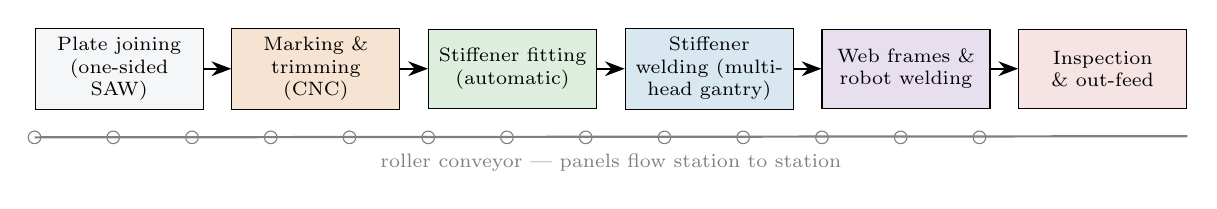
\begin{tikzpicture}[every node/.style={font=\scriptsize}, node distance=0.35cm,
			st/.style={process, minimum width=1.9cm, text width=1.9cm, minimum height=1.0cm}]
			\node[st, fill=cGrayBg] (a) {Plate joining (one-sided SAW)};
			\node[st, right=of a, fill=cOrange!18] (b) {Marking \& trimming (CNC)};
			\node[st, right=of b, fill=cGreen!15] (c) {Stiffener fitting (automatic)};
			\node[st, right=of c, fill=cAccent!15] (d) {Stiffener welding (multi-head gantry)};
			\node[st, right=of d, fill=cPurple!15] (e) {Web frames \& robot welding};
			\node[st, right=of e, fill=cRed!12] (f) {Inspection \& out-feed};
			\draw[flowarrow] (a) -- (b); \draw[flowarrow] (b) -- (c); \draw[flowarrow] (c) -- (d); \draw[flowarrow] (d) -- (e); \draw[flowarrow] (e) -- (f);
			\draw[thick, gray] ($(a.south west)+(0,-0.35)$) -- ($(f.south east)+(0,-0.35)$);
			\foreach \x in {0,1,...,12} \draw[gray] ($(a.south west)+(\x*1.0,-0.35)$) circle (0.08);
			\node[gray, below] at ($(c.south)!0.5!(d.south)+(0,-0.45)$) {roller conveyor --- panels flow station to station};
		\end{tikzpicture}
		\vspace{0.3cm}
		\begin{columns}[T]
			\begin{column}{0.5\textwidth}
				\begin{itemize}\small
					\item A \textbf{flow line} for flat panels (e.g.\ 20 m $\times$ 20 m).
					\item Panels move; equipment stays --- the product layout.
					\item Gantry robots get their weld paths \textbf{from the CAD model}.
				\end{itemize}
			\end{column}
			\begin{column}{0.5\textwidth}
				\begin{block}{Typical results}
					\small Several times the productivity of manual assembly, far less distortion (controlled heat input), and consistent weld quality.
				\end{block}
			\end{column}
		\end{columns}
	\end{frame}

	\begin{frame}{How a Portable Welding Robot Works: The Cell Cycle}
		\vspace*{-0.3cm}
		\begin{block}{The Place---Sense---Weld---Move cycle}
			Like the CPU's machine cycle, a portable robot repeats one cycle for every
			\textbf{double-bottom cell} (a box formed by floors and girders) until the block is finished.
		\end{block}
		\begin{columns}[T]
			\begin{column}{0.55\textwidth}
				\begin{enumerate}\small
					\item \textbf{Place} --- crane or operator puts the robot into the next cell.
					\item \textbf{Sense} --- touch-sensing with the wire finds the real plate edges.
					\item \textbf{Adapt} --- program from CAD is corrected to the measured geometry.
					\item \textbf{Weld} --- all fillet welds in the cell, with arc seam tracking.
					\item \textbf{Check \& move} --- report welds done, lift robot to the next cell.
				\end{enumerate}
			\end{column}
			\begin{column}{0.45\textwidth}
				\centering
				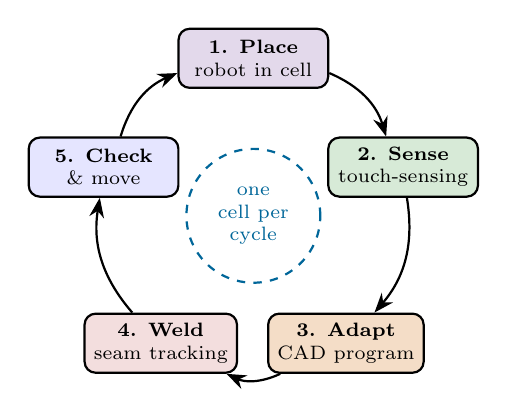
\begin{tikzpicture}[font=\scriptsize,
					stage/.style={rectangle, rounded corners=4pt, draw=black, thick,
						minimum width=1.9cm, minimum height=0.75cm, align=center}]
					\node[circle, draw=cAccent, thick, dashed, minimum size=1.7cm, align=center, text=cAccent]
					(c) at (0,0) {one\\ cell per\\ cycle};
					\node[stage, fill=cPurple!18] (p) at (90:2.0)   {\textbf{1. Place}\\ robot in cell};
					\node[stage, fill=cGreen!18]  (s) at (18:2.0)   {\textbf{2. Sense}\\ touch-sensing};
					\node[stage, fill=cOrange!22] (a) at (-54:2.0)  {\textbf{3. Adapt}\\ CAD program};
					\node[stage, fill=cRed!15]    (w) at (-126:2.0) {\textbf{4. Weld}\\ seam tracking};
					\node[stage, fill=blue!10]    (m) at (162:2.0)  {\textbf{5. Check}\\ \& move};
					\draw[flowarrow] (p) to[bend left=25] (s);
					\draw[flowarrow] (s) to[bend left=25] (a);
					\draw[flowarrow] (a) to[bend left=25] (w);
					\draw[flowarrow] (w) to[bend left=25] (m);
					\draw[flowarrow] (m) to[bend left=25] (p);
				\end{tikzpicture}
			\end{column}
		\end{columns}
	\end{frame}

	\begin{frame}{Welding Robot Technologies}
		\begin{columns}[T]
			\begin{column}{0.5\textwidth}
				\begin{block}{Off-line programming (OLP)}
					\small Weld paths, torch angles and parameters are generated \textbf{automatically from the 3-D model} --- essential because every panel is different. Teaching by pendant would take longer than welding.
				\end{block}
				\begin{block}{Seam finding \& tracking}
					\small \textbf{Touch sensing} (wire touches the plate), \textbf{arc sensing} (current changes during weaving), \textbf{laser line scanners} --- correct for fit-up gaps and distortion.
				\end{block}
			\end{column}
			\begin{column}{0.5\textwidth}
				\centering
				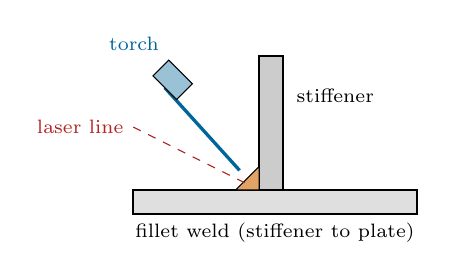
\begin{tikzpicture}[font=\scriptsize]
					% fillet joint
					\filldraw[fill=gray!25, thick] (0,0) rectangle (3.6,0.3);
					\filldraw[fill=gray!40, thick] (1.6,0.3) rectangle (1.9,2.0);
					\filldraw[fill=cOrange!60] (1.6,0.3) -- (1.3,0.3) -- (1.6,0.6) -- cycle;
					% torch
					\draw[very thick, cAccent] (0.4,1.6) -- (1.35,0.55);
					\filldraw[fill=cAccent!40] (0.25,1.75) -- (0.55,1.45) -- (0.75,1.65) -- (0.45,1.95) -- cycle;
					\draw[dashed, cRed] (0.0,1.1) -- (1.5,0.35);
					\node[cRed, left] at (0.0,1.1) {laser line};
					\node[below] at (1.8,0) {fillet weld (stiffener to plate)};
					\node[right] at (1.95,1.5) {stiffener};
					\node[cAccent, above left] at (0.45,1.95) {torch};
				\end{tikzpicture}
				\vspace{0.2cm}
				\begin{itemize}\small
					\item \textbf{Multi-robot gantries} weld both sides of a stiffener at once --- less distortion.
					\item \textbf{Weld data logging} gives traceable quality records for class societies.
				\end{itemize}
			\end{column}
		\end{columns}
	\end{frame}

	\begin{frame}[fragile, plain]{}

		\vspace*{0.05cm}

		\begin{columns}[T,onlytextwidth]

			% =========================================================
			% LEFT COLUMN -- PSEUDOCODE
			% =========================================================

			\begin{column}{0.26\textwidth}

				\begin{block}{Pseudocode}
					\scriptsize
					\begin{enumerate}
						\item START
						\item Set speeds \& arc-on factors: manual 0.3 m/min, 30\,\%; robot 0.5 m/min, 80\,\%
						\item READ weld length \texttt{L}
						\item \texttt{t = L / (v * f) / 60} for each method (hours)
						\item PRINT both times
						\item PRINT \% time saved
						\item STOP
					\end{enumerate}
				\end{block}

			\end{column}


			% =========================================================
			% MIDDLE COLUMN -- C PROGRAM
			% =========================================================
			\hspace*{0.3cm}
			\begin{column}{0.47\textwidth}

				\begin{block}{C Program (welding time)}

\begin{lstlisting}[style=cstyle,numbers=none,basicstyle=\ttfamily\scriptsize]
#include <stdio.h>

int main(void)
{
	float L;                        /* metres */
	float v_man = 0.3, f_man = 0.30; /* m/min */
	float v_rob = 0.5, f_rob = 0.80;
	float t_man, t_rob;

	printf("Enter weld length (m): ");
	scanf("%f", &L);

	t_man = L / (v_man * f_man) / 60.0; /* h */
	t_rob = L / (v_rob * f_rob) / 60.0;

	printf("Manual : %.1f h\n", t_man);
	printf("Robot  : %.1f h\n", t_rob);
	printf("Time saved = %.1f %%\n",
	       100.0 * (1.0 - t_rob / t_man));
	return 0;
}
\end{lstlisting}

				\end{block}

			\end{column}


			% =========================================================
			% RIGHT COLUMN -- OUTPUT
			% =========================================================

			\begin{column}{0.25\textwidth}

				\begin{tikzpicture}[remember picture,overlay]
					\node[
					anchor=north east,
					draw,
					rounded corners=2pt,
					fill=white,
					text width=3.5cm,
					align=left,
					inner sep=6pt
					] at ([xshift=-2mm,yshift=-6mm]current page.north east)
					{
						\textbf{Program Output}\\[3pt]
						\ttfamily\scriptsize
						Enter weld length (m): 200\\
						Manual : 37.0 h\\
						Robot  : 8.3 h\\
						Time saved = 77.5 \%
					};
				\end{tikzpicture}

			\end{column}

		\end{columns}

		\begin{tikzpicture}[remember picture,overlay]
			\node[
			anchor=south east,
			draw,
			rounded corners=2pt,
			fill=cGrayBg,
			text width=3.5cm,
			align=left,
			inner sep=6pt,
			font=\scriptsize
			] at ([xshift=-2mm,yshift=4mm]current page.south east)
			{
				\textbf{Check by hand} ($L = 200$ m):\\
				Manual: $\dfrac{200}{0.3\times0.3} = 2222$ min $= 37.0$ h\\[2pt]
				Robot: $\dfrac{200}{0.5\times0.8} = 500$ min $= 8.3$ h\\[3pt]
				Most of the gain comes from the higher \textbf{arc-on time}, not the higher speed.
			};
		\end{tikzpicture}

	\end{frame}

	% =================================================================
	\section{Robots in Blasting and Painting}
	% =================================================================
	\begin{frame}{Surface Preparation and Painting in Shipbuilding}
		\begin{columns}[T]
			\begin{column}{0.5\textwidth}
				\begin{block}{Why it matters}
					\small Coating protects the hull and tanks from corrosion for 15--25 years. Rules such as IMO \textbf{PSPC} (ballast tanks) demand surface cleanliness (e.g.\ Sa 2\,\textonehalf), profile and dry-film thickness (DFT) --- consistently.
				\end{block}
				\begin{block}{Why automate it}
					\begin{itemize}\small
						\item Abrasive dust, silica, noise, solvent fumes --- serious \textbf{health hazards}.
						\item Huge areas (tens of thousands of m$^2$ per ship).
						\item Uniform DFT is hard to achieve by hand.
					\end{itemize}
				\end{block}
			\end{column}
			\begin{column}{0.5\textwidth}
				\renewcommand{\arraystretch}{1.25}
				\centering
				\small
				\begin{tabular}{@{}>{\raggedright}p{2.4cm}>{\raggedright\arraybackslash}p{3.4cm}@{}}
					\toprule
					\textbf{Stage} & \textbf{Automated equipment} \\
					\midrule
					Plate / profile & shot-blast \& priming line (fixed automation) \\
					Blocks          & blasting \& painting robots in enclosed halls \\
					Hull in dock    & boom / gantry robots, magnetic crawlers \\
					Repair \& maintenance & UHP water-jetting crawlers, hull-cleaning ROVs \\
					\bottomrule
				\end{tabular}
			\end{column}
		\end{columns}
	\end{frame}

	\begin{frame}{Blasting and Painting Robots}
		\begin{columns}[T]
			\begin{column}{0.55\textwidth}
				\begin{itemize}\small
					\item \textbf{Magnetic crawlers} climb the steel hull and carry a blasting or UHP water-jet head; debris is vacuumed back (closed loop, no dust cloud).
					\item \textbf{Boom / gantry painting robots} spray the hull side in the dock with constant stand-off distance and speed.
					\item \textbf{Block painting robots} in halls with ventilation and temperature control.
					\item Sensors measure stand-off, overlap and wet-film thickness; data logged for inspectors.
				\end{itemize}
			\end{column}
			\begin{column}{0.45\textwidth}
				\centering
				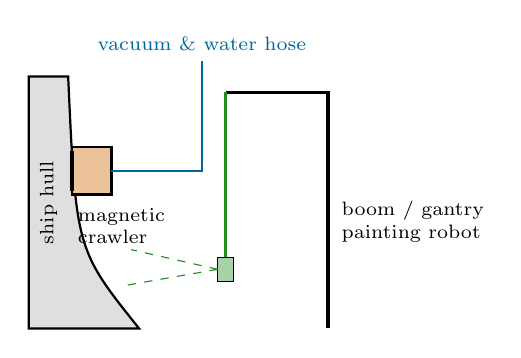
\begin{tikzpicture}[font=\scriptsize]
					% hull side
					\filldraw[fill=gray!25, thick] (0,0) -- (0,3.2) -- (0.5,3.2) .. controls (0.6,1.0) .. (1.4,0) -- cycle;
					\node[rotate=90] at (0.25,1.6) {ship hull};
					% crawler
					\filldraw[fill=cOrange!40, thick] (0.55,1.7) rectangle (1.05,2.3);
					\draw[very thick] (0.55,1.75) -- (0.55,2.25);
					\draw[thick, cAccent] (1.05,2.0) -- (2.2,2.0) -- (2.2,3.4) node[above] {vacuum \& water hose};
					\node[below right, align=left] at (0.5,1.65) {magnetic\\ crawler};
					% gantry painter
					\draw[very thick] (3.8,0) -- (3.8,3.0) -- (2.5,3.0);
					\draw[very thick, cGreen] (2.5,3.0) -- (2.5,0.9);
					\filldraw[fill=cGreen!40] (2.4,0.9) rectangle (2.6,0.6);
					\draw[cGreen, dashed] (2.4,0.75) -- (1.25,0.55) (2.4,0.75) -- (1.3,1.0);
					\node[right] at (3.85,1.5) {boom / gantry};
					\node[right] at (3.85,1.2) {painting robot};
				\end{tikzpicture}
			\end{column}
		\end{columns}
		\vspace{0.1cm}
		\footnotesize\centering Robots keep the gun at a constant distance, angle and speed --- the three things that decide film thickness.
	\end{frame}

	\begin{frame}{Painting: Worked Example on Paint Consumption}
		\begin{block}{Paint volume needed}
			\[
			V_{\text{paint}} = \frac{A \times \text{DFT}}{\text{VS} \times \text{TE}}
			\]
			$A$ = area, DFT = dry-film thickness, VS = volume solids of the paint, TE = transfer efficiency (fraction reaching the surface).
		\end{block}
		\begin{columns}[T]
			\begin{column}{0.5\textwidth}
				\textbf{Problem:} a hull area of 5000 m$^2$ gets one coat of DFT 250 $\mu$m, paint VS $= 60\,\%$. Manual spraying reaches TE $= 60\,\%$; a robot reaches TE $= 85\,\%$. How much paint is saved?
			\end{column}
			\begin{column}{0.5\textwidth}
				\small
				\begin{align*}
					A\cdot\text{DFT} &= 5000\times250\times10^{-6} = 1.25\ \text{m}^3\\
					V_{\text{man}} &= \frac{1.25}{0.6\times0.6} = 3.47\ \text{m}^3 \approx 3472\ \text{L}\\
					V_{\text{rob}} &= \frac{1.25}{0.6\times0.85} = 2.45\ \text{m}^3 \approx 2451\ \text{L}\\
					\text{Saving} &\approx \boxed{1021\ \text{L}\ (29\,\%)}
				\end{align*}
			\end{column}
		\end{columns}
		\vspace{0.1cm}
		\footnotesize\centering Less overspray also means less solvent emission and cleaner air in the dock.
	\end{frame}

	% =================================================================
	\section{Heavy Lifting and Handling}
	% =================================================================
	\begin{frame}{Heavy Lifting in the Shipyard}
		\begin{columns}[T]
			\begin{column}{0.5\textwidth}
				\begin{itemize}\small
					\item \textbf{Goliath (gantry) cranes} over the building dock --- lift blocks of several hundred to 1000+ tonnes.
					\item \textbf{Block turn-over} --- two hooks rotate a block so it can be welded down-hand.
					\item \textbf{Self-propelled modular transporters (SPMT)} --- computer-steered multi-axle trailers move blocks between shops.
					\item \textbf{Automated plate stock-yards} --- magnet cranes pick plates by ID.
				\end{itemize}
			\end{column}
			\begin{column}{0.5\textwidth}
				\centering
				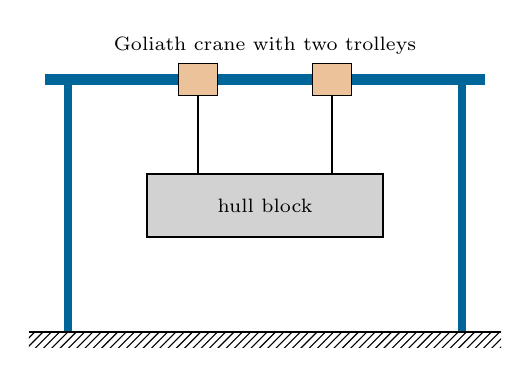
\begin{tikzpicture}[font=\scriptsize]
					% goliath crane
					\draw[line width=3pt, cAccent] (0,0) -- (0,3.2);
					\draw[line width=3pt, cAccent] (5,0) -- (5,3.2);
					\draw[line width=4pt, cAccent] (-0.3,3.2) -- (5.3,3.2);
					\filldraw[fill=cOrange!40] (1.4,3.0) rectangle (1.9,3.4);
					\filldraw[fill=cOrange!40] (3.1,3.0) rectangle (3.6,3.4);
					\draw[thick] (1.65,3.0) -- (1.65,2.0);
					\draw[thick] (3.35,3.0) -- (3.35,2.0);
					% block
					\filldraw[fill=gray!35, thick] (1.0,1.2) rectangle (4.0,2.0);
					\node at (2.5,1.6) {hull block};
					% dock
					\fill[pattern=north east lines] (-0.5,-0.2) rectangle (5.5,0);
					\draw[thick] (-0.5,0) -- (5.5,0);
					\node[above] at (2.5,3.4) {Goliath crane with two trolleys};
				\end{tikzpicture}
				\vspace{0.1cm}

				\footnotesize Automation: synchronised hoisting, anti-sway control, load monitoring, laser positioning.
			\end{column}
		\end{columns}
	\end{frame}

	\begin{frame}{Heavy Lifting: Worked Examples}
		\begin{columns}[T]
			\begin{column}{0.5\textwidth}
				\begin{block}{Tandem (two-hook) lift}
					\small A 300 t block hangs from hooks A and B, 20 m apart. Its centre of gravity is 8 m from A. Find the hook loads.
				\end{block}
				\small
				\begin{align*}
					R_A &= W\,\frac{12}{20} = 300\times0.6 = \boxed{180\ \text{t}}\\
					R_B &= W\,\frac{8}{20} = 300\times0.4 = \boxed{120\ \text{t}}
				\end{align*}
				\footnotesize The hook \textbf{nearer} the CG carries more; each hoist must stay within its rating.
			\end{column}
			\begin{column}{0.5\textwidth}
				\centering
				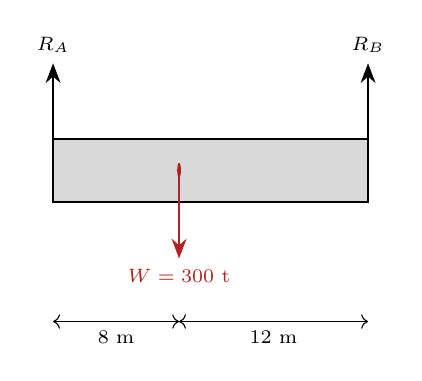
\begin{tikzpicture}[font=\scriptsize, x=0.2cm, y=0.8cm]
					\filldraw[fill=gray!30, thick] (0,0) rectangle (20,1.0);
					\draw[flowarrow] (0,1.0) -- (0,2.2) node[above] {$R_A$};
					\draw[flowarrow] (20,1.0) -- (20,2.2) node[above] {$R_B$};
					\draw[flowarrow, cRed] (8,0.5) -- (8,-0.9) node[below] {$W = 300$ t};
					\fill[cRed] (8,0.5) circle (0.12);
					\draw[<->] (0,-1.9) -- (8,-1.9) node[midway, below] {8 m};
					\draw[<->] (8,-1.9) -- (20,-1.9) node[midway, below] {12 m};
				\end{tikzpicture}
				\vspace{0.2cm}
				\begin{block}{SPMT axle load}
					\small 600 t block, 24 axle lines: $600/24 = \boxed{25\ \text{t/axle line}}$, levelled hydraulically by the transporter's computer.
				\end{block}
			\end{column}
		\end{columns}
	\end{frame}

	% =================================================================
	\section{Automation of Other Tasks}
	% =================================================================
	\begin{frame}{Automation of Other Shipyard Tasks}
		\renewcommand{\arraystretch}{1.08}
		\centering
		\footnotesize
		\begin{tabular}{@{}>{\raggedright}p{2.8cm}>{\raggedright}p{5.0cm}>{\raggedright\arraybackslash}p{4.8cm}@{}}
			\toprule
			\textbf{Task} & \textbf{Automation} & \textbf{Benefit} \\
			\midrule
			Plate cutting \& marking & CNC plasma, oxy-fuel, laser; ink-jet marking & accurate parts, nested to save steel \\
			Plate bending   & CNC press, automated line heating         & less skill-dependent forming \\
			Pipe fabrication & robotic cutting, bending, orbital welding & high-quality spools, labels from CAD \\
			Inspection      & automated UT, 3-D laser scanning, drones in tanks & fast, safe, digital records \\
			Logistics       & RFID tracking, AGVs, automated warehouses & right part at the right time \\
			Worker support  & exoskeletons, AR glasses, cobots          & less fatigue \& injury \\
			\bottomrule
		\end{tabular}
		\vspace{0.1cm}
		\begin{block}{Beyond the yard}
			\small Automation also runs the ship itself: unmanned machinery spaces, integrated bridge systems, dynamic positioning and, increasingly, \textbf{autonomous vessels}.
		\end{block}
	\end{frame}

	\begin{frame}{Accuracy Control with 3-D Scanning and Drones}
		\begin{columns}[T]
			\begin{column}{0.5\textwidth}
				\begin{block}{Accuracy control}
					\small Blocks must fit at erection within a few millimetres. A 3-D laser scanner or total station measures the finished block; software compares it with the CAD model and predicts the fit \textbf{before} the block is lifted.
				\end{block}
				\begin{itemize}\small
					\item Less cutting and re-fitting in the dock.
					\item Shrinkage data fed back to design (added margins).
				\end{itemize}
			\end{column}
			\begin{column}{0.5\textwidth}
				\begin{block}{Drones \& crawlers for inspection}
					\small Drones with cameras and ultrasonic probes inspect tanks, cargo holds and hull areas that would otherwise need scaffolding --- faster and safer surveys.
				\end{block}
				\centering
				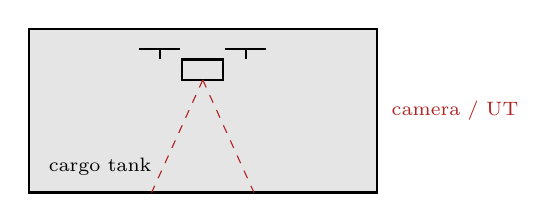
\begin{tikzpicture}[font=\scriptsize, scale=1.3]
					\draw[thick, fill=gray!20] (0,0) rectangle (3.4,1.6);
					\node[right] at (0.1,0.25) {cargo tank};
					\draw[thick] (1.5,1.1) rectangle (1.9,1.3);
					\foreach \dx in {-0.35,0.35} {
						\draw[thick] (1.7+\dx*1.2,1.3) -- (1.7+\dx*1.2,1.4);
						\draw[thick] (1.7+\dx*1.2-0.2,1.4) -- (1.7+\dx*1.2+0.2,1.4);
					}
					\draw[dashed, cRed] (1.7,1.1) -- (1.2,0.0) (1.7,1.1) -- (2.2,0.0);
					\node[cRed, right] at (3.45,0.8) {camera / UT};
				\end{tikzpicture}
			\end{column}
		\end{columns}
	\end{frame}

	\begin{frame}{Summary \& What Comes Next}
		\begin{columns}[T]
			\begin{column}{0.5\textwidth}
				\begin{block}{Concept}
					\begin{itemize}\small
						\item Manufacturing concepts \& production metrics.
						\item Reasons for automating; USA principle.
						\item Types of production \& plant layouts in a shipyard.
						\item Types of automation, strategies, migration.
						\item Levels of automation in shipbuilding.
						\item Digital shipyards, product model, digital twin.
						\item Robots in welding, blasting, painting, lifting \& other tasks.
					\end{itemize}
				\end{block}
			\end{column}
			\begin{column}{0.5\textwidth}
				\begin{block}{Practice makes perfect}
					\begin{itemize}\small
						\item Re-work the MLT, welding-time, paint and lifting examples with new data.
						\item Run the welding-time C program for other weld lengths and arc-on factors.
						\item List the automation you would add first in a small shipyard, and why.
					\end{itemize}
				\end{block}
				\begin{block}{Coming up}
					\small Marine automation on board: engine-room automation, integrated bridge systems and autonomous ships.
				\end{block}
			\end{column}
		\end{columns}
	\end{frame}

	%------------------------------------------------
	\begin{frame}
		\centering
		\Huge Thank You
		\vspace{0.5cm}

		\normalsize Questions?
	\end{frame}

	%------------------------------------------------

\end{document}
